\subsubsection{模型的建立}
\textbf{1.马尔可夫性质的引入} 

在本题中，因为玩家仅知道当天的天气状况，并需要据此决定当天的行动方案，
%
所以过去的天气对当下已经没有任何参考价值。
%
那么天气随机的限制可简化为在每一天中只知道当前的天气状态，同时通过预测下一天的天气来帮助玩家进行下一步的决策，
%
根据该天气性质，可以引入马尔科夫性来解决此问题：
%
即下一状态只依赖于当前状态，与过去状态无关。以下给出马尔可夫的数学表达式：
\begin{align}
P\bigl(X_{n+1}=x \mid X_1=x_1, X_2=x_2, \dots, X_n=x_n\bigr) = P\bigl(X_{n+1}=x \mid X_n=x_n\bigr)
\end{align}

\textbf{2.引入马尔可夫后的决策过程} 

在玩家决策时，不仅要考虑天气的外部因素，还需要考虑自身负重、行走天数、水和食物等内部因素，
%
不同的未来天气会让玩家做出不同的决策。所以要建立基于马尔可夫性质的决策方程：
\begin{align}
F = \bigl(D_t,~I, ~G_t\bigr)
\end{align}

其中，$D_t$为第t天的天气， $I$为内部因素（包括自身负重、行走天数、水和食物），
%
$G_t$为在$D$这个天气序列下在第t天的剩余资金。

\textbf{3.约束条件的界定} 

在题目中，首先要保证在规定的时间内到达终点，其次才是保留尽可能多的资金。
%
所以我们应该优先考虑能否走到终点。
%
即我们应该在起点买足所有的水和食物，以确保在最坏的天气情况下可以到达村庄或终点来补充物资：
\begin{align}
T_t \geqslant 0, F_t \geqslant 0
\end{align}

其中，$S$为从起点到村庄或终点的路径。

\textbf{4.具有马尔可夫性质的模型总结} 

基于以上分析，我们可写出最后的具有马尔可夫性质的最大化收益决策模型：
\begin{align}
F = \{ F(t) \mid F(t) \text{ 为基于 } (D_t, I) \text{ 算出来的最大化收益} \}
\end{align}

整合即得：
\[
\begin{aligned}
\max_{} \quad & F(t) \\
\text{s.t.} \quad & 0 \le t \le 30, \\
& G_t \ge 0,\; F_t \ge 0,\; T_t \ge 0, \quad t = 0,1,\dots,30, \\
& 0 < M_t \le M_{\max}, \quad t = 0,1,\dots,30, \\
& D_t = 3 \implies N_t = N_{t-1}, \quad t = 1,\dots,30.
\end{aligned}
\]

\subsubsection{模型的求解及结果}

\textbf{动态规划求解} 

\textbf{1.数据初始化}
根据表格数据初始化各天气的食物和水的消耗和路线，设定每个状态的最大收益为无穷小。
%
同时根据第一天的天气给出初始水和食物的购买方案。

\textbf{2.约束条件的补充}

动态规划算法必须当前一步有解才能进行下一步的状态转移，所以我们要确定在不同天气序列下的解的范围。

在每个状态下，都先从最坏的情况下进行考虑，假设后面全部都是高温，从而获得一个能走到终点的结果，
%
即所有解的下界。

\textbf{3.动态规划的求解}

利用跟问题一相同的动态规划算法求解。

\textbf{4.结果线路的输出}

利用dfs回溯法来反向寻找经过路线。

根据以上流程来进行第三关，第四关的求解。

\textbf{结果呈现和分析}

\textbf{1.第三关结果呈现}

由于第三关仅有晴朗和高温两种天气情况，所以我们采用二叉决策树来表现在每一个点上的决策和状态变化。结果如下图。\\

\begin{figure}[H]
    \centering
    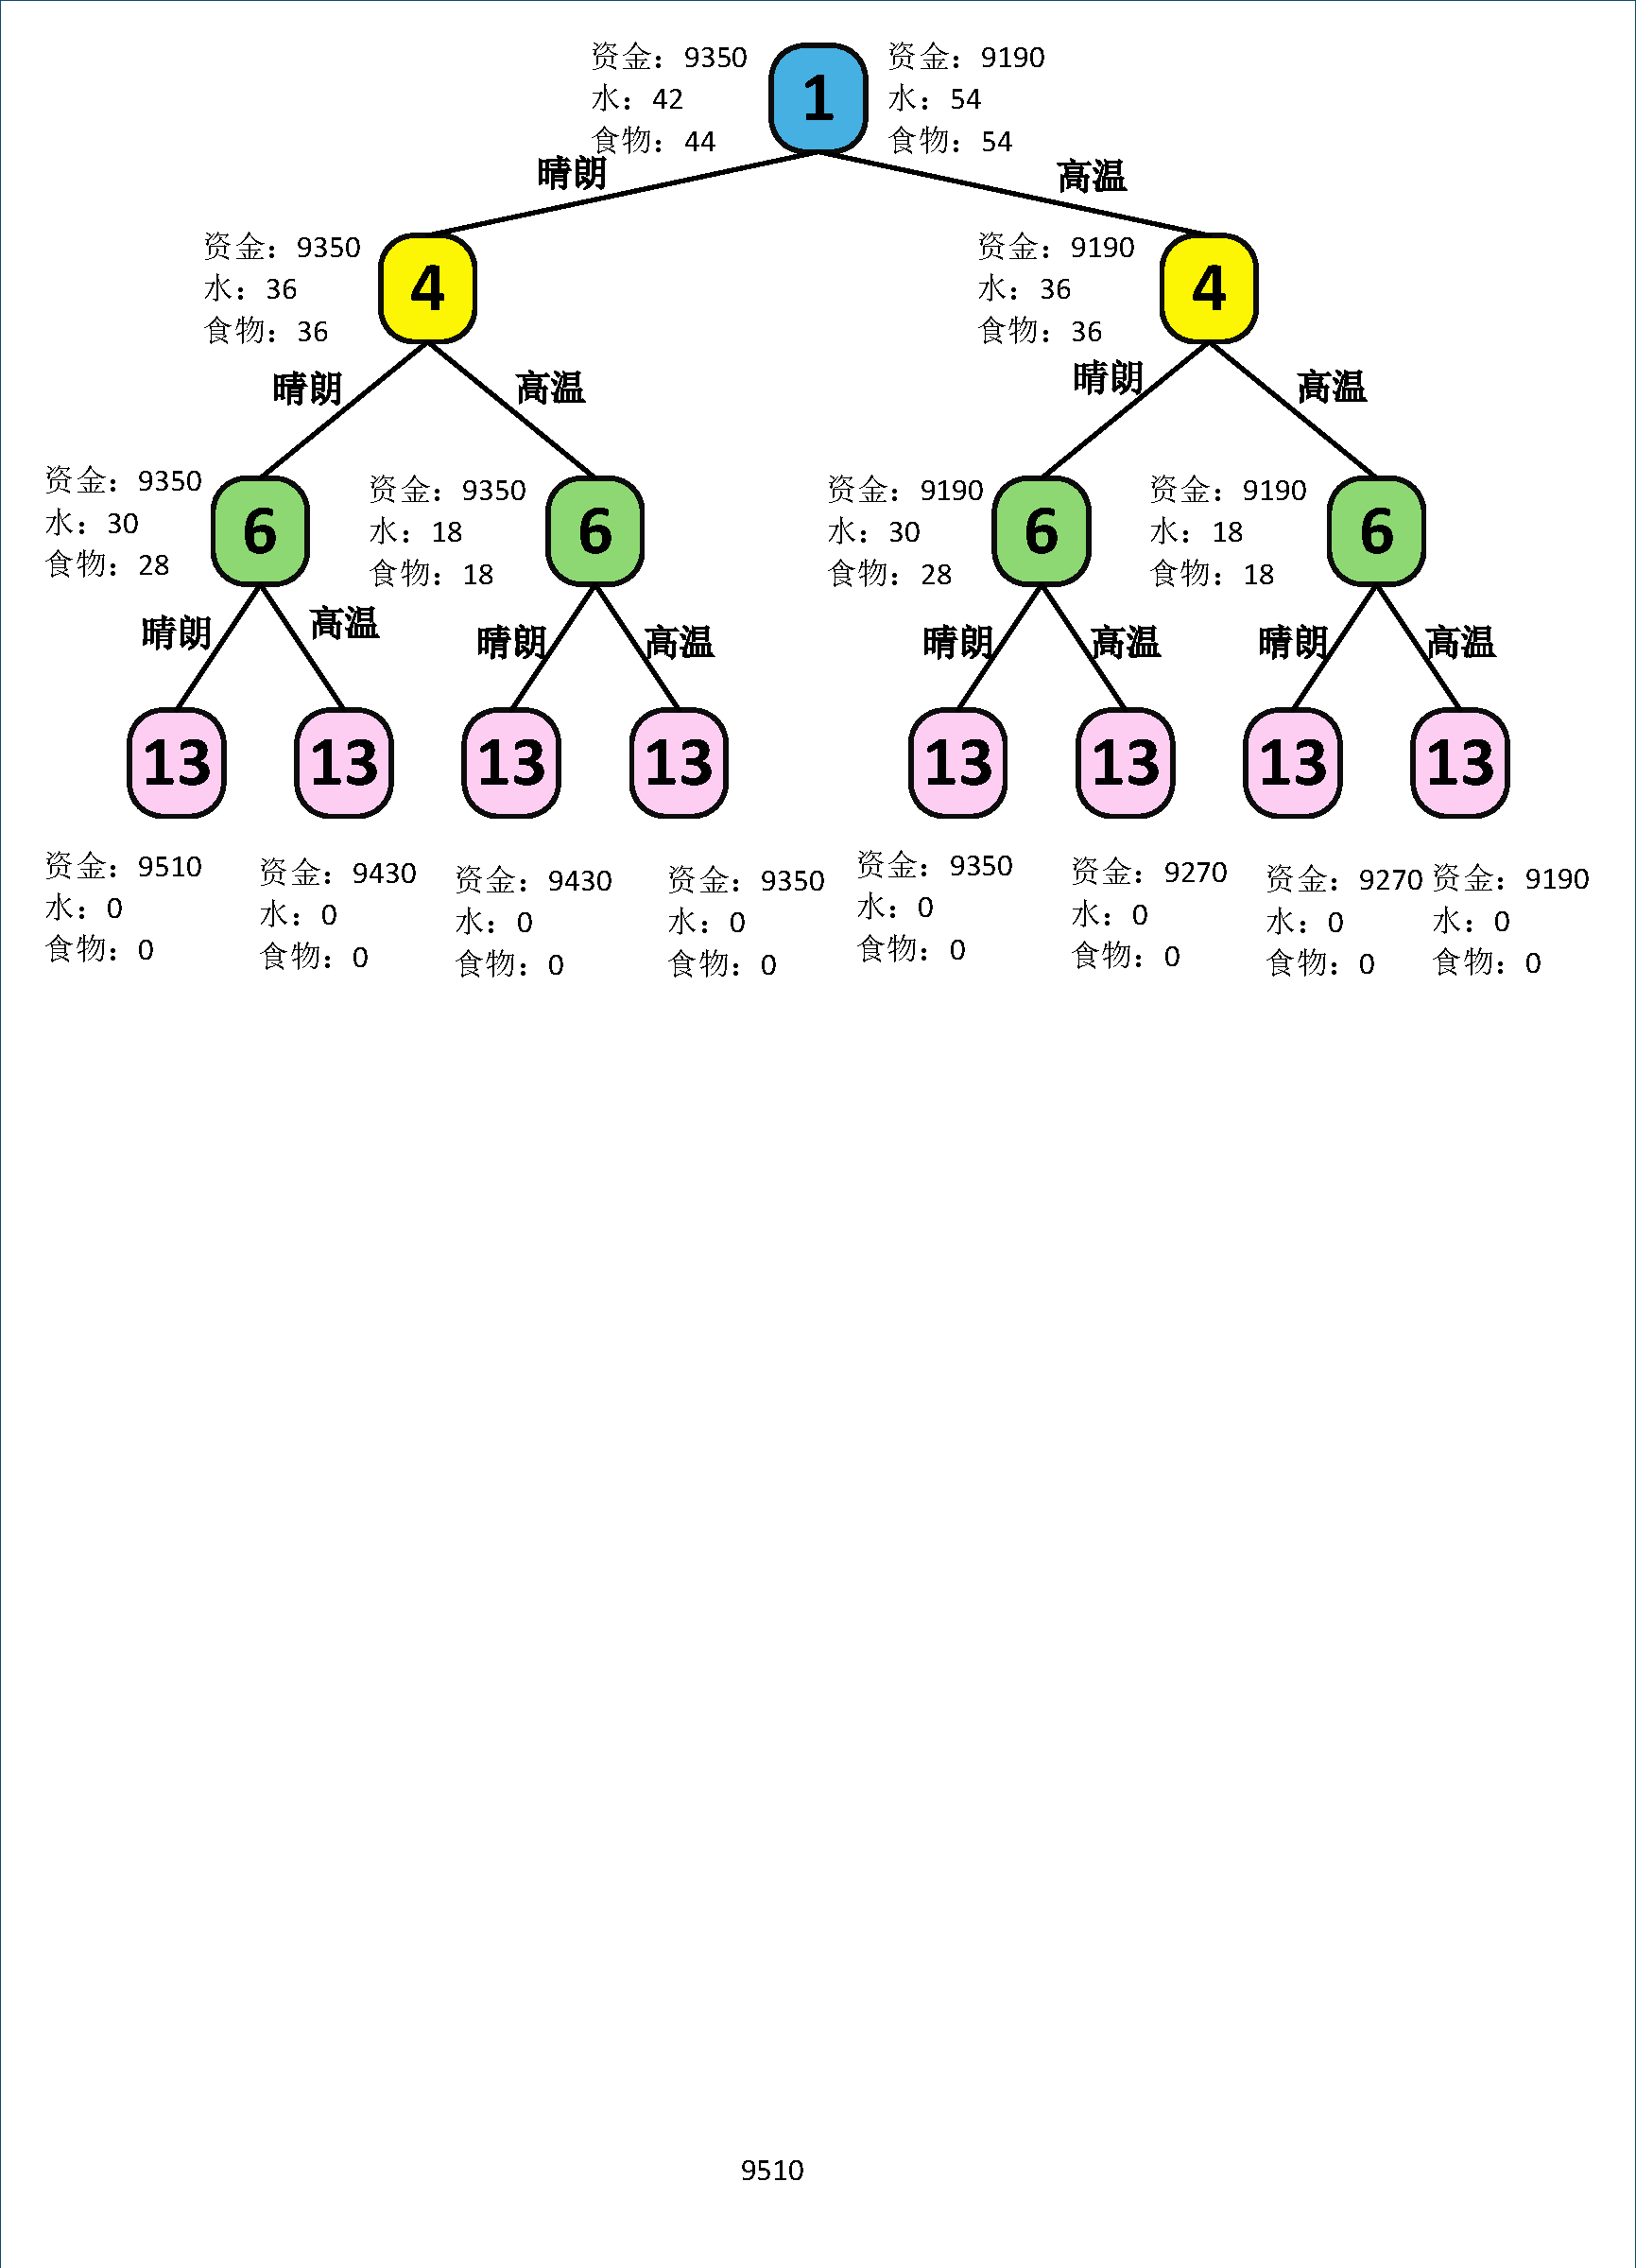
\includegraphics[width=0.8\textwidth]{C2020b/figure/第三关结果图.pdf}
    \caption{第三关结果图}
\end{figure}

我们可以发现路线均是从$1->4->6->13$。说明在该沙漠的地图下，通过如上的决策得到的最优解相同，所以该决策具有稳定性。

\textbf{2.第四关结果呈现}

由于第四关存在晴朗，高温和沙暴三种天气情况，且到终点的最少天数也需要10天，所以使用二叉决策树会使得结果冗余。故采用画图法来展示结果\\

与第三关相同在每个状态下，都先从最坏的情况下进行考虑，假设后面全部都是高温，中间小概率随机插入沙暴天气，从而获得一个能走到终点的结果，即所有解的下界\\

如下是其中一种可能的路线结果：

\begin{figure}[H]
    \centering
    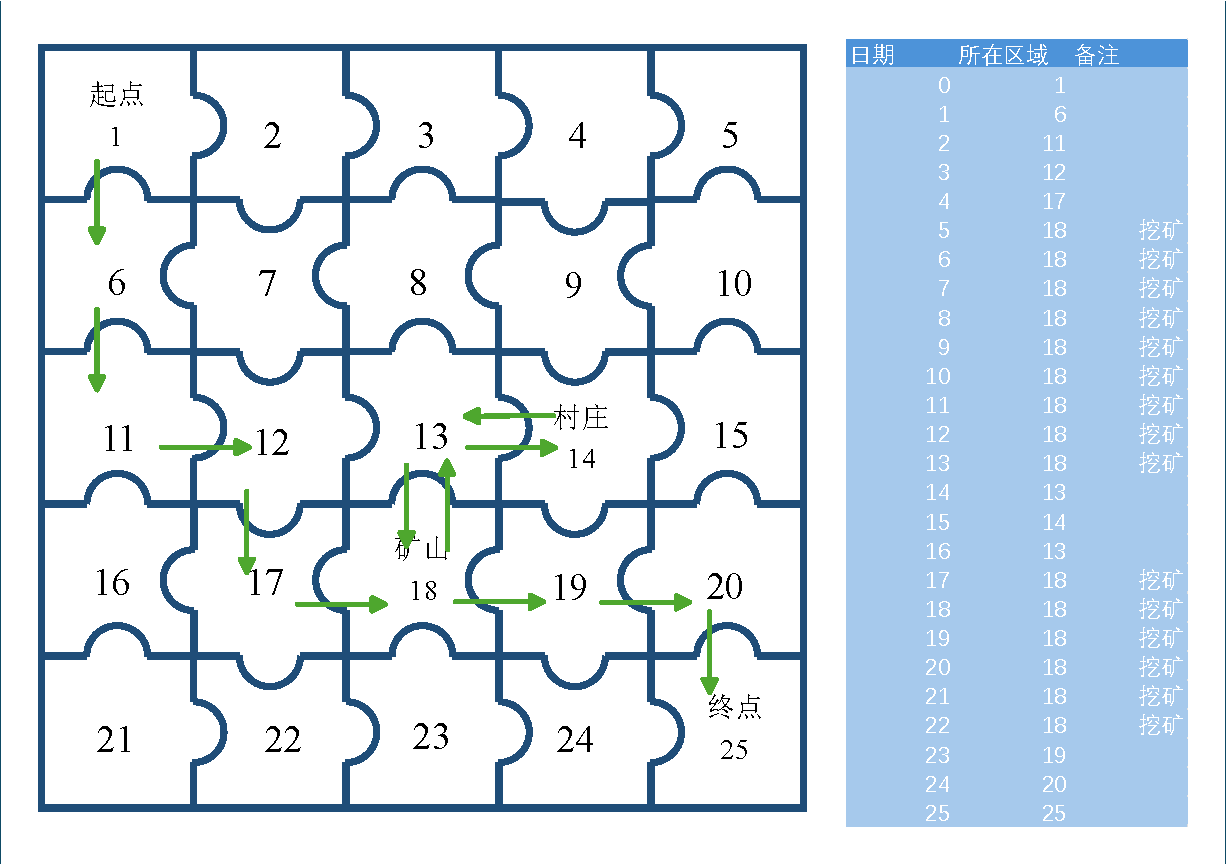
\includegraphics[width=0.8\textwidth]{C2020b/figure/第四关结果图.pdf}
    \caption{第四关结果图}
\end{figure}

所有时刻的各种状态如下：\\

\begin{figure}[h]
\centering
\begin{subfigure}[t]{0.48\textwidth}
\centering
\renewcommand{\arraystretch}{1.2}
\begin{tabular}{|c|c|c|c|c|}
\hline
天数 & 当前位置 & 当前水 & 当前食物 & 利润 \\
\hline
0 & 1 & 196 & 305 & 5970 \\
1 & 6 & 190 & 297 & 5970 \\
2 & 11 & 184 & 289 & 5970 \\
3 & 12 & 178 & 281 & 5970 \\
4 & 17 & 172 & 273 & 5970 \\
5 & 18 & 166 & 265 & 5970 \\
6 & 18 & 157 & 253 & 6970 \\
7 & 18 & 130 & 226 & 7970 \\
8 & 18 & 103 & 199 & 8970 \\
9 & 18 & 94 & 187 & 9970 \\
10 & 18 & 85 & 175 & 10970 \\
11 & 18 & 76 & 163 & 11970 \\
12 & 18 & 67 & 151 & 12970 \\
\hline
\end{tabular}
\end{subfigure}
\hfill
\begin{subfigure}[t]{0.48\textwidth}
\centering
\renewcommand{\arraystretch}{1.2}
\begin{tabular}{|c|c|c|c|c|}
\hline
天数 & 当前位置 & 当前水 & 当前食物 & 利润 \\
\hline
13 & 18 & 40 & 124 & 13970 \\
14 & 13 & 22 & 106 & 14970 \\
15 & 14 & 225 & 225 & 15970 \\
16 & 13 & 219 & 217 & 16970 \\
17 & 18 & 213 & 209 & 17970 \\
18 & 18 & 186 & 182 & 17970 \\
19 & 18 & 159 & 155 & 17710 \\
20 & 18 & 132 & 128 & 16860 \\
21 & 18 & 105 & 101 & 16860 \\
22 & 18 & 96 & 89 & 17860 \\
23 & 19 & 90 & 81 & 17860 \\
24 & 20 & 84 & 73 & 17860 \\
25 & 25 & 78 & 65 & 17860 \\
\hline
\end{tabular}
\end{subfigure}
\end{figure}

